
\documentclass[12pt]{article}
\title{CISC 102 (Fall 20)\\ Homework \#9: Relations $\;$   (31 Points) }
\author{Student Name/ID: Artie Lomonaco/20216334}
\date{}


\usepackage[left=2cm, right=3cm, top=1cm]{geometry}

\usepackage{amsmath}
\usepackage{amsfonts}
\usepackage{amssymb}
\usepackage{amsthm}
\usepackage{bm}						% for \bm -- bold almost everywhere
\usepackage{mdwlist}					% for {itemize*}
\usepackage{enumerate}
\usepackage{xcolor,graphicx}
\usepackage{relsize,etoolbox}
\usepackage{tikz}

\newcommand{\abs}[1]{\left| #1 \right|}
\newcommand{\ab}[1]{\left[ #1 \right]}
\newcommand{\rb}[1]{\left( #1 \right)}
\newcommand{\set}[1]{\left\{ #1 \right\}}
\newcommand{\norm}[1]{\left\| #1 \right\|}
\newcommand{\wt}[1]{\widetilde{#1}}
\newcommand{\pdif}[2]{\frac{\partial #1 }{\partial #2}}
\newcommand{\pdifm}[3]{\frac{\partial^{#3} #1 }{\partial #2^{#3}}}

\renewcommand{\a}{\ensuremath{\mathcal{A}}}
\renewcommand{\b}{\ensuremath{\mathcal{B}}}
\newcommand{\bb}{\ensuremath{\mathbb{B}}}
\newcommand{\ee}{\ensuremath{\mathbb{E}}}
\newcommand{\f}{\ensuremath{\mathcal{F}}}
\newcommand{\g}{\ensuremath{\mathcal{G}}}
\newcommand{\h}{\ensuremath{\mathcal{H}}}
\renewcommand{\l}{\ensuremath{\mathcal{L}}}
\newcommand{\map}{\longrightarrow}
\newcommand{\nn}{\ensuremath{\mathbb{N}}}
\newcommand{\one}{\ensuremath{\mathbf{1}}}
\newcommand{\p}{\ensuremath{\mathcal{P}}}
\newcommand{\pp}{\ensuremath{\mathbb{P}}}
\newcommand{\qq}{\ensuremath{\mathbb{Q}}}
\newcommand{\rr}{\ensuremath{\mathbb{R}}}
\newcommand{\zz}{\ensuremath{\mathbb{Z}}}

\let\oldemptyset\emptyset
\let\emptyset\varnothing

\newcommand{\var}{\mathrm{var}}

\DeclareMathOperator{\argmax}{argmax}

\begin{document}

\maketitle


\begin{enumerate}

\item (6 pts)
Let $R$ be the relation on the natural numbers defined by
\[ R = \{(x, y): x, y \in \mathbb{N}, x^2 + y^2 \leq 8\}.\]
\begin{enumerate}
	\item Write out the elements of $R$ as a set of ordered pairs\\
    \\$(0,0),(0,1),(0,2),(1,0),(1,1),(1,2),(2,0),(2,1),(2,2)$
	\item Is $R$ an equivalence relation, and explain why or why not?\\
    \\ $R$ is reflexive since it contains the pairs of form $(a,a)$ which are elements $(0,0),(1,1),(2,2)$. $R$ is symmetrical since $(a,b) \in R$ and $(b,a) \in R$. $R$ is transitive since $\forall a \forall b \forall c (((a,b) \in R \land (b.c) \in R) \rightarrow (a,c) \in R)$ which are illustrated in all the pairs.
	\item Is $R$ a partial order and explain why or why not?\\
    \\It is not a partial order since this function is an equivalence function, which means that it is symmetric. For a function to be a partial order it needs to be reflexive, transitive, and antisymmetric. A function can't be both symmetric and antisymmetric, and since $R$ is already symmetric it cannot be a partial order.
\end{enumerate}
%%%
\item (2 pts) \\
Let A be a set with \(n\) elements, and let B be a set with \(m\) elements  ( \(n \ge 0 , m \ge 0\) )
\leavevmode\\\relax
How many relations are there from A to B?\\
\\We know that $A \times B$ has $nm$ number of elements when $A$ has $n$ elements and $B$ has $m$ elements. A set with $k$ number of elements has $2^k$ number of subsets, $\therefore$ there are $2^{n\times m}$ relations on two sets with $n$ and $m$ elements, which are $A$ and $B$.

\item (4 pts)
Let \(A\) be a set and let \(R\) and \(S\) be relations on \(A\).
\begin{enumerate}
\item  Suppose \(R\) is anti-symmetric. Prove that \(R \cap S\) is also anti-symmetric.\\
\\A relation is antisymmetric if $\forall a \forall b (((a,b) \in R \land (b,a) \in R) (a = b))$
\\Suppose that $T = R \cap S$. If $(a,b)$ is in $T$ and also $(b,a)$ is in $T$, if shows that both $(a,b)$ and $(b,a)$ are in $R$ since $T \subseteq R$, because $T = R\cap S$. From this, since $R$ is anti symmetric, we arrive at $a=b$. $\therefore$ We conclude that $T$ is antisymmetric.
\item Suppose \(R\) and \(S\) are both transitive. Prove that \(R \cap S\) is also transitive.
\\Let $(a,b),(b,c) \in R \cap S$
\\$\rightarrow (a,b),(b,c) \in R$ and $(a,b),(b,c) \in S$
\\$\rightarrow (a,c) \in R $ and $(a,c) \in S$ (Since both $R$ and $S$ are transitive)
\\$(a,c)\in R \cap S$
\\$\therefore$ we conclude that $R \cap S$ is transitive if both $R$ and $S$ are transitive.
\end{enumerate}
%%%
\item (2 pts)
Let \(A = \lbrace{1,2,3,4,5,6,7,8,9,10,11,12,13,14,15}\rbrace\) \\
Let \(R\) be the relation on \(A\) defined by\\
\((a,b)\in R \text{ if and only if } b=a+3m\) for some non-negative integer \(m\)
\\
For example, \((5,11)\in R \text{ because } 11=5+3 \cdot 2\)
\\
Is \(R\) a partial ordering on \(A\)? Prove your answer.\\
\\First by looking at the formula we can see that this relation is reflexive since it contains all the pairs in the form of $(a,a)$  since $b = a \times (m)(0) \rightarrow a = a$. We can also see that this relation is antisymmetric since there are no pairs of elements $a$ and $b$ with a $a \neq b$ such that both $(a,b)$ and $(b,a)$ belong to the relation. We can see with the example given above; $11 = 5 + 3\times 2$ but $5 = 11 + 3\times m$ but $m$ must be negative for equality to hold but it cannot. This relation is also transitive since we see that for one of many examples $5 = 2 + 3\times 1$ so we sub it into the example given $11 = (2 + 3 \times 1) + 3 \times 2 = 2 + 3 \times 3 = 11$. $\therefore$ from all this we conclude that this function is a partial ordering since it is reflexive, antisymmetric and transitive.

\item (2 pts)
Let \(R\) be a relation defined on the set \(\lbrace 0,1,2,3,\dots \rbrace\) as follows:
\leavevmode\\\relax
\(\hspace{50pt} (a,b) \in R\) if and only if \((a+b)\) is a multiple of 2
\leavevmode\\\relax
(a) is R reflexive?\\
\\$R$ is reflexive since a number plus itself is a multiple of 2 whether it is even or odd. to show this we let a even integer = $2k$ and on odd integer = $2k-1$. $2k + 2k = 4k = 2(2k)$, and $(2k-1) + (2k-1) = 4k-2 = 2(2k-2) $, so we can see that this relation is indeed reflexive since an integer added to itself will result in a multiple of 2.\\
\leavevmode\\\relax
(b) is R symmetric?\\
\\This relation is also symmetric because if you add two integers together and form a multiple of two, you can have the pair in any order $(a,b)$ or $(b,a)$ since it doesn't matter in what order they are added in. $\therefore$ this relation is also symmetric.

\item (6 pts)
Let $A = \{0, 1, 2, 3, 4\}$ and define a relation $R$ on $A$ as follows:
\[R = \{(0, 0), (0, 4), (1, 1), (1, 3), (2, 2), (3, 1), (3, 3), (4, 0), (4, 4)\}.\]
\begin{enumerate}
	\item Draw the directed graph of $R$\\
    \begin{center}
    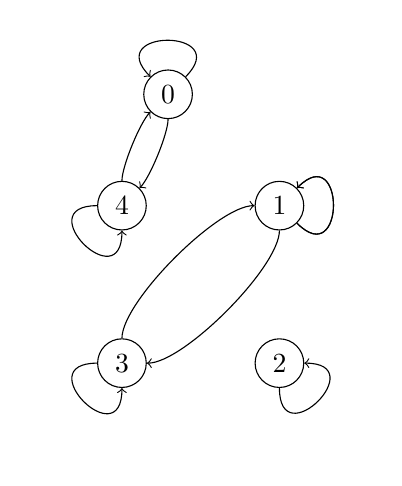
\begin{tikzpicture}[node distance={20mm}, main/.style = {draw, circle}]
    \node[main] (1) {0};
    \node[main] (2) [below right of=1] {1};
    \node[main] (3) [below of=2] {2};
    \node[main] (4) [left of=3] {3};
    \node[main] (5) [above of=4] {4};
    \draw[->] (1) to [out=45,in=135,looseness=5] (1);
    \draw[->] (1) to [out=270,in=45,looseness=0.5] (5);
    \draw[->] (2) to [out=315,in=45,looseness=5] (2);
    \draw[->] (2) to [out=270,in=360,looseness=0.5] (4);
    \draw[->] (3) to [out=270,in=360,looseness=5] (3);
    \draw[->] (2) to [out=315,in=45,looseness=5] (2);
    \draw[->] (4) to [out=90,in=180,looseness=0.5] (2);
    \draw[->] (4) to [out=180,in=270,looseness=5] (4);
    \draw[->] (5) to [out=90,in=225,looseness=0.5] (1);
    \draw[->] (5) to [out=180,in=270,looseness=5] (5);
    \end{tikzpicture}
    \end{center}
	\item Find the equivalence class of every element of $A.$
    \\$[0] = \{0,4\}$
    \\$[1] = \{1,3\}$
    \\$[2] = \{2\}$
    \\$[3] = \{1,3\}$
    \\$[4] = \{0,4\}$
	\item Find  the distinct equivalence classes of the relation (Usually several of the classes 	will contain exactly the same elements, so you must take a careful look at the classes to determine which are the same. You then indicate the distinct equivalence 	classes by describing them without duplication.)\\
\\The distinct equivalence classes in this relation would be $\{0,4\,\{1,3\},\{2\}$ does not include the duplicates.
\end{enumerate}


\item (5 pts) \\
Which of these relations on $\{0, 1, 2, 3\}$ are equivalence relations? For those that are not, what  properties do they lack?
\begin{enumerate}[(i)]
	\item $\{ 0 \sim 0 , 1 \sim 1 , 2 \sim 2 , 3 \sim 3\}$
	\\This relation is not a equivalence relation since each it is only transitive since each element is only related to itself. This relation lacks the properties of being transitive.
	\item $\{ 0 \sim 0 , 0 \sim 2 , 2 \sim 0 , 2 \sim 2 , 2 \sim 3 , 3 \sim 2 , 3 \sim 3\}$
	\\This relation is an equivalence relation.
	\item $\{ 0 \sim 0 , 1 \sim 1 , 1 \sim 2 , 2 \sim 1 , 2 \sim 2 , 3 \sim 3\}$
	\\This relation is not an equivalence relation. 1 and 2 are related to each other but are not related to 0 in any way. We see that this relation is reflexive, but it is not symmetric or transitive.
	\item $\{ 0 \sim 0 , 1 \sim 1 , 1 \sim 3 , 2 \sim 2 , 2 \sim 3 , 3 \sim 1 , 3 \sim 2 , 3 \sim 3\}$
	\\This relation is also not an equivalence relation. It lacks the property of being symmetric and transitive.

	\item $\{ 0 \sim 0 , 0 \sim 1 , 0 \sim 2 , 1 \sim 0 , 1 \sim 1 , 1 \sim 2 , 2 \sim 0 , 2 \sim 2 , 3 \sim 3\}$
    \\This is an equivalence relation.
\end{enumerate}	


\item (4 pts) \\
For the following relations on $A$ determine whether they are reflexive, symmetric, and/or transitive. State whether they are equivalence relations or not, and if they are describe their equivalence classes.
\begin{enumerate}
	\item Let $A=\mathbb{Z}$ and define $\sim$ by $a\sim b$ whenever  $a- b$ is odd.\\
    \\First we show that an odd number minus an odd number (2k - 1 -(2k - 1) =0)and the same case with even numbers (2k - 2k = 0) equal to an even integer This function is not reflexive since $a-a =0$ and 0 is an even number. This function is symmetric since it doesn't matter in what order two numbers are subtracted, they will result in an odd number. This is shown in these to examples: $2k - (2k - 1) = 1$ and $(2k - 1) - 2k = -1$ and both these results result in odd numbers, but these two numbers bust be one odd and one even for this to occur. This function is transitive since every set of pairs of integers can be transposed with another and result in an odd subtraction. $\therefore$ this function is symmetric and transitive.
	\item Let $A=\mathbb{R}$ and define $\sim$ by $a\sim b$ whenever $ab \neq 0$.\\
    \\This relation is reflexive, symmetric and transitive, and it contains all real numbers exempt for 0. It's reflexive since $a\times a$ is not equal to 0 if $a \neq 0$. It is symmetric since it does not matter in what order you multiply two numbers, they will result in the same result and not equal to 0 unless one or both of them is 0. It is transitive too since any number times any number is not equal to 0. $\therefore$ we see that this relation is an equivalence relation since it is reflexive, symmetric, and transitive.
\end{enumerate}	
	
%%%%%%%%%%%%%%%%



\vfill
\end{enumerate}
\end{document}
